\documentclass[14pt,ignorenonframetext,aspectratio = 1610]{beamer}
\setbeamertemplate{caption}[numbered]
\setbeamertemplate{caption label separator}{: }
\setbeamercolor{caption name}{fg=normal text.fg}
\beamertemplatenavigationsymbolsempty
\usepackage{lmodern}
\usepackage{amssymb,amsmath}
\usepackage{ifxetex,ifluatex}
\usepackage{fixltx2e} % provides \textsubscript
\ifnum 0\ifxetex 1\fi\ifluatex 1\fi=0 % if pdftex
\usepackage[T1]{fontenc}
\usepackage[utf8]{inputenc}
\else % if luatex or xelatex
\ifxetex
\usepackage{mathspec}
\else
\usepackage{fontspec}
\fi
\defaultfontfeatures{Ligatures=TeX,Scale=MatchLowercase}
\setmainfont[]{Roboto}
\setmonofont[Mapping=tex-ansi]{Lucida Console}
\fi
\usefonttheme{serif} % use mainfont rather than sansfont for slide text
% use upquote if available, for straight quotes in verbatim environments
\IfFileExists{upquote.sty}{\usepackage{upquote}}{}
% use microtype if available
\IfFileExists{microtype.sty}{%
\usepackage{microtype}
\UseMicrotypeSet[protrusion]{basicmath} % disable protrusion for tt fonts
}{}
\newif\ifbibliography
\usepackage{color}
\usepackage{fancyvrb}
\newcommand{\VerbBar}{|}
\newcommand{\VERB}{\Verb[commandchars=\\\{\}]}
\DefineVerbatimEnvironment{Highlighting}{Verbatim}{commandchars=\\\{\}}
% Add ',fontsize=\small' for more characters per line
\usepackage{framed}
\definecolor{shadecolor}{RGB}{248,248,248}
\newenvironment{Shaded}{\begin{snugshade}}{\end{snugshade}}
\newcommand{\KeywordTok}[1]{\textcolor[rgb]{0.13,0.29,0.53}{\textbf{{#1}}}}
\newcommand{\DataTypeTok}[1]{\textcolor[rgb]{0.13,0.29,0.53}{{#1}}}
\newcommand{\DecValTok}[1]{\textcolor[rgb]{0.00,0.00,0.81}{{#1}}}
\newcommand{\BaseNTok}[1]{\textcolor[rgb]{0.00,0.00,0.81}{{#1}}}
\newcommand{\FloatTok}[1]{\textcolor[rgb]{0.00,0.00,0.81}{{#1}}}
\newcommand{\ConstantTok}[1]{\textcolor[rgb]{0.00,0.00,0.00}{{#1}}}
\newcommand{\CharTok}[1]{\textcolor[rgb]{0.31,0.60,0.02}{{#1}}}
\newcommand{\SpecialCharTok}[1]{\textcolor[rgb]{0.00,0.00,0.00}{{#1}}}
\newcommand{\StringTok}[1]{\textcolor[rgb]{0.31,0.60,0.02}{{#1}}}
\newcommand{\VerbatimStringTok}[1]{\textcolor[rgb]{0.31,0.60,0.02}{{#1}}}
\newcommand{\SpecialStringTok}[1]{\textcolor[rgb]{0.31,0.60,0.02}{{#1}}}
\newcommand{\ImportTok}[1]{{#1}}
\newcommand{\CommentTok}[1]{\textcolor[rgb]{0.56,0.35,0.01}{\textit{{#1}}}}
\newcommand{\DocumentationTok}[1]{\textcolor[rgb]{0.56,0.35,0.01}{\textbf{\textit{{#1}}}}}
\newcommand{\AnnotationTok}[1]{\textcolor[rgb]{0.56,0.35,0.01}{\textbf{\textit{{#1}}}}}
\newcommand{\CommentVarTok}[1]{\textcolor[rgb]{0.56,0.35,0.01}{\textbf{\textit{{#1}}}}}
\newcommand{\OtherTok}[1]{\textcolor[rgb]{0.56,0.35,0.01}{{#1}}}
\newcommand{\FunctionTok}[1]{\textcolor[rgb]{0.00,0.00,0.00}{{#1}}}
\newcommand{\VariableTok}[1]{\textcolor[rgb]{0.00,0.00,0.00}{{#1}}}
\newcommand{\ControlFlowTok}[1]{\textcolor[rgb]{0.13,0.29,0.53}{\textbf{{#1}}}}
\newcommand{\OperatorTok}[1]{\textcolor[rgb]{0.81,0.36,0.00}{\textbf{{#1}}}}
\newcommand{\BuiltInTok}[1]{{#1}}
\newcommand{\ExtensionTok}[1]{{#1}}
\newcommand{\PreprocessorTok}[1]{\textcolor[rgb]{0.56,0.35,0.01}{\textit{{#1}}}}
\newcommand{\AttributeTok}[1]{\textcolor[rgb]{0.77,0.63,0.00}{{#1}}}
\newcommand{\RegionMarkerTok}[1]{{#1}}
\newcommand{\InformationTok}[1]{\textcolor[rgb]{0.56,0.35,0.01}{\textbf{\textit{{#1}}}}}
\newcommand{\WarningTok}[1]{\textcolor[rgb]{0.56,0.35,0.01}{\textbf{\textit{{#1}}}}}
\newcommand{\AlertTok}[1]{\textcolor[rgb]{0.94,0.16,0.16}{{#1}}}
\newcommand{\ErrorTok}[1]{\textcolor[rgb]{0.64,0.00,0.00}{\textbf{{#1}}}}
\newcommand{\NormalTok}[1]{{#1}}

% Prevent slide breaks in the middle of a paragraph:
\widowpenalties 1 10000
\raggedbottom

\AtBeginPart{
\let\insertpartnumber\relax
\let\partname\relax
\frame{\partpage}
}
\AtBeginSection{
\ifbibliography
\else
\let\insertsectionnumber\relax
\let\sectionname\relax
\frame{\sectionpage}
\fi
}
\AtBeginSubsection{
\let\insertsubsectionnumber\relax
\let\subsectionname\relax
\frame{\subsectionpage}
}

\setlength{\parindent}{0pt}
\setlength{\parskip}{6pt plus 2pt minus 1pt}
\setlength{\emergencystretch}{3em}  % prevent overfull lines
\providecommand{\tightlist}{%
\setlength{\itemsep}{0pt}\setlength{\parskip}{0pt}}
\setcounter{secnumdepth}{0}
\usepackage{fontspec}
\usepackage{fontawesome}
\newfontfamily{\FA}{FontAwesome}
%\usepackage[table,x11names]{xcolor}
%\usepackage{hyperref}
%\hypersetup{colorlinks, urlcolor = magenta}
\usepackage{color, colortbl}
\definecolor{SpringGreen}{rgb}{0, 1, 0.498}
\definecolor{brightpink}{rgb}{1.0, 0.0, 0.5}
\newcommand{\R}{\textbf{\textsf{R}}}

\title{Accessing and Analyzing\\
MLB Pitch Tracking Data in R}
\author{Aaron R. Baggett, Ph.D.}
\institute{University of Mary Hardin-Baylor\\
Department of Psychology}
\date{March 28, 2017}

\begin{document}
\frame{\titlepage}

\begin{frame}{Resources}

\begin{itemize}
\tightlist
\item
  Slides, data, and R code are available at:
\end{itemize}

\begin{center}
\color{brightpink}\Large{\texttt{bit.ly/austin\_r}}
\end{center}

\end{frame}

\section{\texorpdfstring{Major League Baseball (MLB)
\protect \newline Pitch Tracking
Data}{Major League Baseball (MLB) Pitch Tracking Data}}\label{major-league-baseball-mlb-pitch-tracking-data}

\begin{frame}{MLB Pitch Tracking Data}

\begin{itemize}
\tightlist
\item
  Since 2007, MLB has tracked pitch location and play-by-play data for
  all games
\item
  Source: Sportvision PITCHf/x system
\item
  PITCHf/x data are fed real time to mobile and desktop apps
\item
  All data are stored in XML format on MLB servers
\end{itemize}

\end{frame}

\begin{frame}{MLB Pitch Tracking Data}

\begin{itemize}
\tightlist
\item
  Location:
  \color{brightpink}\url{http://gd2.mlb.com/components/game/mlb/}
\end{itemize}

\vspace{-1mm}\begin{center}
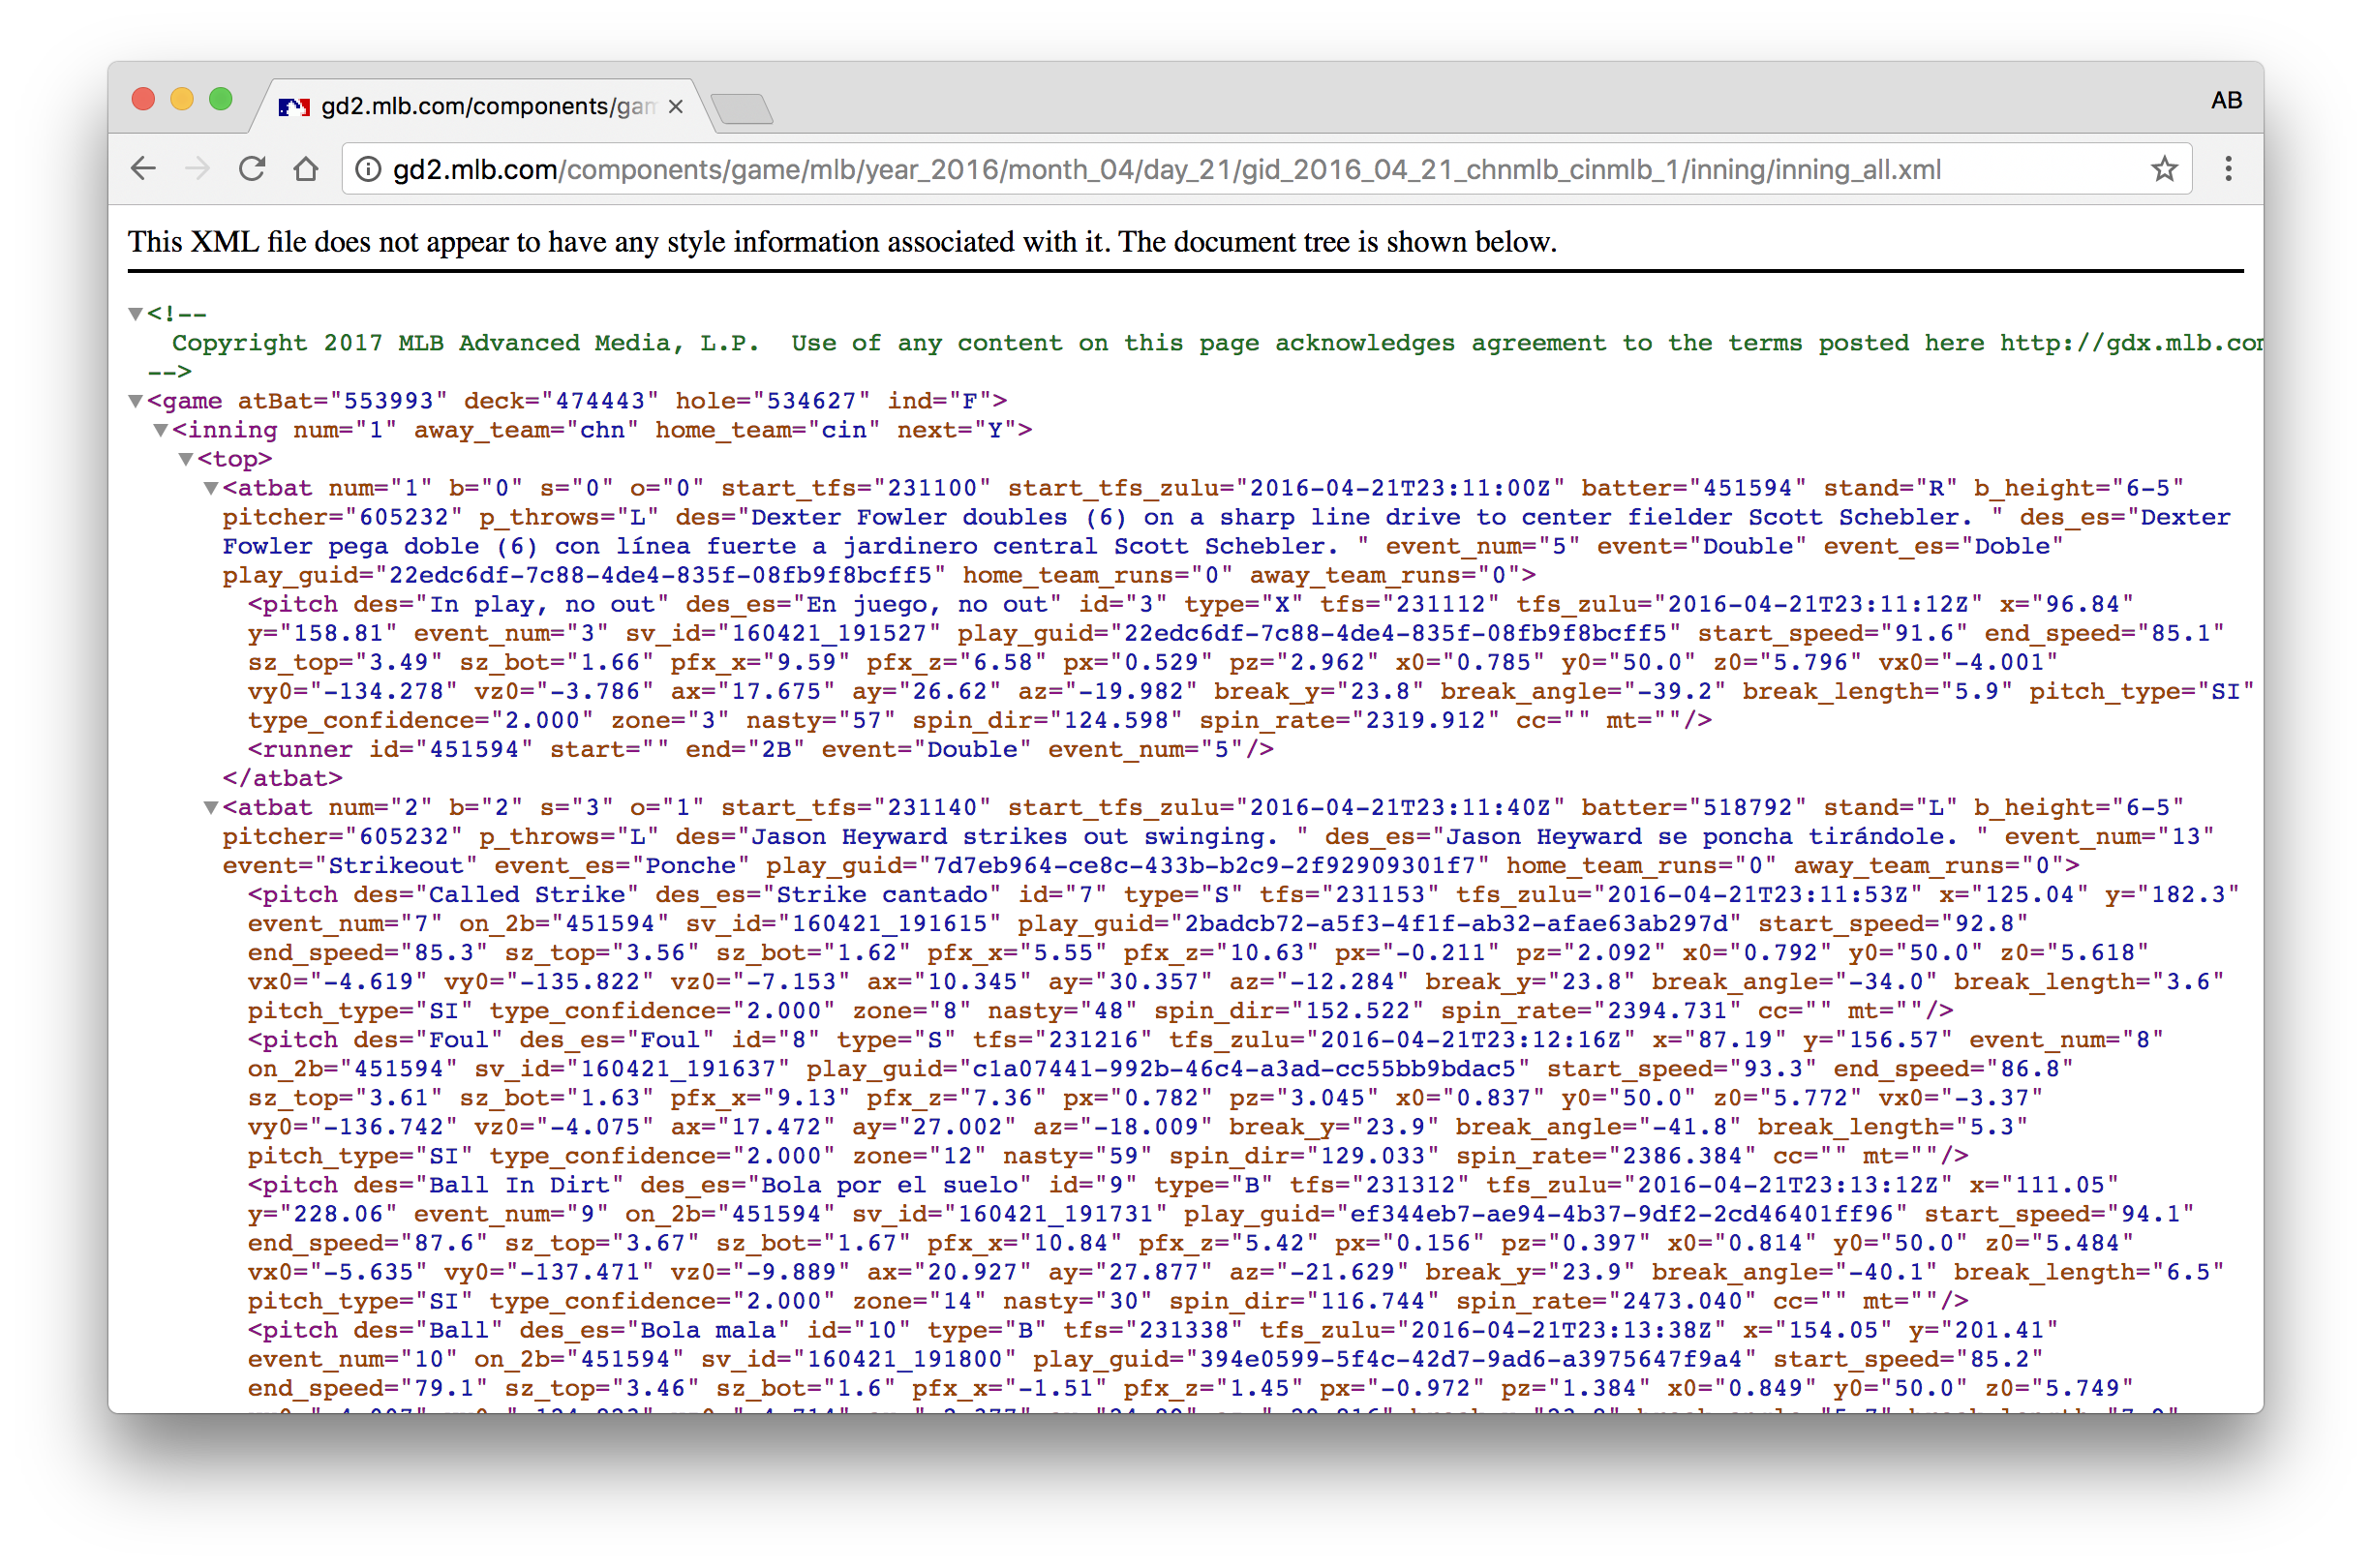
\includegraphics[width = 4.5in]{../figs/gd_inning_all.png}
\end{center}

\end{frame}

\section{Accessing MLB Pitch Tracking
Data}\label{accessing-mlb-pitch-tracking-data}

\begin{frame}[fragile]{Accessing MLB Pitch Tracking Data}

\begin{itemize}
\tightlist
\item
  R packages:

  \begin{enumerate}
  \def\labelenumi{\arabic{enumi}.}
  \tightlist
  \item
    \emph{\texttt{pitchRx}}: Data collection
  \item
    \emph{\texttt{dplyr}}: Data analysis
  \end{enumerate}
\end{itemize}

\end{frame}

\begin{frame}[fragile]{\texttt{pitchRx}}

\begin{itemize}
\tightlist
\item
  Prior to 2013, researchers had to scrape PITCHf/x data manually
\item
  In 2013, Carson Sievert created the \emph{\texttt{pitchRx}} R package
\item
  \emph{\texttt{pitchRx}} contains tools for accessing play-by-play data
\end{itemize}

\end{frame}

\begin{frame}[fragile]{\texttt{pitchRx}}

\begin{itemize}
\tightlist
\item
  Prior to 2013, researchers had to scrape PITCHf/x data manually
\item
  In 2013, Carson Sievert created the \emph{\texttt{pitchRx}} R package
\item
  \emph{\texttt{pitchRx}} contains tools for accessing play-by-play data
\end{itemize}

\footnotesize

\begin{Shaded}
\begin{Highlighting}[]
\NormalTok{pfx_db <-}\StringTok{ }\KeywordTok{src_sqlite}\NormalTok{(}\StringTok{"pfx_db.sqlite3"}\NormalTok{, }\DataTypeTok{create =} \OtherTok{TRUE}\NormalTok{)}
\NormalTok{files <-}\StringTok{ }\KeywordTok{c}\NormalTok{(}\StringTok{"inning/inning_all.xml"}\NormalTok{, }\StringTok{"players.xml"}\NormalTok{, }\StringTok{"miniscoreboard.xml"}\NormalTok{)}
\KeywordTok{scrape}\NormalTok{(}\DataTypeTok{start =} \StringTok{"YYY-MM-DD"}\NormalTok{, }\DataTypeTok{end =} \StringTok{"YYY-MM-DD"}\NormalTok{, }\DataTypeTok{suffix =} \NormalTok{files, }
  \DataTypeTok{connect =} \NormalTok{pfx_db$con)}
\NormalTok{pfx_db <-}\StringTok{ }\KeywordTok{src_sqlite}\NormalTok{(}\StringTok{"~/your/working/directory/pfx_db.sqlite3"}\NormalTok{)}
\KeywordTok{src_tbls}\NormalTok{(pfx_16)}
\end{Highlighting}
\end{Shaded}

\end{frame}

\begin{frame}{\texttt{pitchRx}}

\begin{itemize}
\tightlist
\item
  Once we set up a PITCHf/x database, we have access to all MLB pitch
  and gameplay data
\item
  Best to use a small date range for initial setup
\item
  10 primary tables in the data
\end{itemize}

\end{frame}

\begin{frame}{PITCHf/x Data Tables}

\small

\begin{table}[ht]
\centering
\begin{tabular}{ll}
\hline
Table Name & Description \\ 
\hline
{\texttt{action}} & Ball/strike count, result of pitch, ... \\ 
{\texttt{atbat}} & Pitcher/batter names, handedness, heights, at bat result, ... \\ 
{\texttt{coach}} & Names of manager and staff, ... \\ 
{\texttt{game}} & Venue, start time, time zone, TV, win-loss records, ... \\ 
{\texttt{media}} & Mobile/TV media assets, ... \\ 
{\texttt{pitch}} & Umpire's decision/outcome, strike zone parameters, x-y coordinates, ... \\ 
{\texttt{player}} & Players' stats, position, number, ... \\ 
{\texttt{po}} & Details about put out attempts (e.g., pickoffs and stolen bases), ... \\ 
{\texttt{runner}} & Details about base runner(s) and at bat events, ... \\ 
{\texttt{umpire}} & Umpire names and positions, ... \\ 
\hline
\end{tabular}
\end{table}

\end{frame}

\begin{frame}{PITCHf/x Data Tables}

For most analyses, we usually work with:

\small

\begin{table}[ht]
\centering
\begin{tabular}{ll}
\hline
Table Name & Description \\ 
\hline
{\texttt{action}} & Ball/strike count, result of pitch, ... \\ 
\rowcolor{SpringGreen}{\texttt{atbat}} & Pitcher/batter names, handedness, heights, at bat result, ... \\ 
{\texttt{coach}} & Names of manager and staff, ... \\ 
{\texttt{game}} & Venue, start time, time zone, TV, win-loss records, ... \\ 
{\texttt{media}} & Mobile/TV media assets, ... \\ 
\rowcolor{SpringGreen}{\texttt{pitch}} & Umpire's decision/outcome, strike zone parameters, x-y coordinates, ... \\ 
{\texttt{player}} & Players' stats, position, number, ... \\ 
{\texttt{po}} & Details about put out attempts (e.g., pickoffs and stolen bases), ... \\ 
{\texttt{runner}} & Details about base runner(s) and at bat events, ... \\ 
\rowcolor{SpringGreen}{\texttt{umpire}} & Umpire names and positions, ... \\ 
\hline
\end{tabular}
\end{table}

\end{frame}

\begin{frame}[fragile]{\texttt{dplyr}}

\begin{itemize}
\tightlist
\item
  Wickham and Francois (2016)
\item
  A grammar of data manipulation
\item
  Provides a set of verbs for lots of tasks

  \begin{itemize}
  \tightlist
  \item
    \emph{\texttt{select()}}: Selects columns
  \item
    \emph{\texttt{filter()}}: Filters rows (e.g., \texttt{==},
    \texttt{!=}, \texttt{\textless{}=}, etc.)
  \item
    \emph{\texttt{arrange()}}: Re-orders and sorts rows
  \item
    \emph{\texttt{mutate()}}: Creates new variables/columns
  \item
    \emph{\texttt{summarise()}}: Summarizes values/output
  \item
    \emph{\texttt{group\_by()}}: Allows for by-group operations
  \end{itemize}
\end{itemize}

\end{frame}

\begin{frame}[fragile]{Accessing MLB Pitch Tracking Data}

\begin{itemize}
\tightlist
\item
  R packages:

  \begin{enumerate}
  \def\labelenumi{\arabic{enumi}.}
  \tightlist
  \item
    \emph{\texttt{pitchRx}}: Data collection
  \item
    \emph{\texttt{dplyr}}: Data analysis
  \end{enumerate}
\end{itemize}

\end{frame}

\section{Analyzing MLB Pitch Tracking
Data}\label{analyzing-mlb-pitch-tracking-data}

\begin{frame}{Tonight}

\begin{itemize}
\tightlist
\item
  There are several ways to analyze PITCHf/x data

  \begin{itemize}
  \tightlist
  \item
    Ex.: Pitching/batting outcomes, predictive models, et al.
  \end{itemize}
\item
  Tonight though, let's concentrate on home plate umpire decisions
\item
  Specifically:

  \begin{enumerate}
  \def\labelenumi{\arabic{enumi}.}
  \tightlist
  \item
    How many pitches do umpires see during games? Of those, how many
    require a decision?
  \item
    How accurate are \emph{all} umpires over the season? How accurate
    are \emph{individual} umpires over the season?
  \end{enumerate}
\end{itemize}

\end{frame}

\begin{frame}{1. Pitches Seen vs.~Decisions Made}

\begin{itemize}
\tightlist
\item
  How many pitches do umpires see during games? Of those, how many
  require an umpire decision?

  \begin{itemize}
  \tightlist
  \item
    \textbf{Pitches seen:} Total number of recorded pitches thrown
    during game
  \item
    \textbf{Decisions made:} Total number of called strikes and called
    balls during game
  \end{itemize}
\end{itemize}

\end{frame}

\begin{frame}[fragile]{1. Pitches Seen vs.~Decisions Made}

\begin{itemize}
\tightlist
\item
  We'll use the \texttt{pitch} table to answer these questions
\item
  Steps:

  \begin{enumerate}
  \def\labelenumi{\arabic{enumi}.}
  \tightlist
  \item
    Create data frame for pitches seen, \emph{\texttt{observed}}
  \item
    Create data frame for decisions made, \emph{\texttt{decisions}}
  \item
    Join \emph{\texttt{observed}} and \emph{\texttt{decisions}}
  \item
    Calculate proportion of pitches requiring decision
  \item
    Calculate simple descriptive statistics
  \end{enumerate}
\end{itemize}

\end{frame}

\begin{frame}[fragile]{1. Pitches Seen vs.~Decisions Made}

\begin{itemize}
\tightlist
\item
  Step 1. Create data frame for pitches seen
\end{itemize}

\footnotesize

\begin{Shaded}
\begin{Highlighting}[]
\NormalTok{observed <-}\StringTok{ }\NormalTok{pitch %>%}\StringTok{ }
\StringTok{  }\KeywordTok{group_by}\NormalTok{(gameday_link) %>%}\StringTok{ }
\StringTok{  }\KeywordTok{summarize}\NormalTok{(}\DataTypeTok{seen =} \KeywordTok{n}\NormalTok{())}
\end{Highlighting}
\end{Shaded}

\end{frame}

\begin{frame}[fragile]{1. Pitches Seen vs.~Decisions Made}

\begin{itemize}
\tightlist
\item
  Step 1. Create data frame for pitches seen
\item
  R code:

  \begin{itemize}
  \tightlist
  \item
    \emph{\texttt{pitch}}: Current data frame
  \item
    \emph{\texttt{group\_by()}}, \emph{\texttt{summarize()}},
    \emph{\texttt{n()}}: \emph{\texttt{dplyr}} verbs
  \item
    \emph{\texttt{gameday\_link}}: Unique date/team label
  \item
    \emph{\texttt{seen}}: New name for variable \texttt{n()}
  \item
    \emph{\texttt{observed}}: Name of new data frame
  \end{itemize}
\end{itemize}

\footnotesize

\begin{Shaded}
\begin{Highlighting}[]
\NormalTok{observed <-}\StringTok{ }\NormalTok{pitch %>%}\StringTok{ }
\StringTok{  }\KeywordTok{group_by}\NormalTok{(gameday_link) %>%}\StringTok{ }
\StringTok{  }\KeywordTok{summarize}\NormalTok{(}\DataTypeTok{seen =} \KeywordTok{n}\NormalTok{())}
\end{Highlighting}
\end{Shaded}

\end{frame}

\begin{frame}[fragile]{1. Pitches Seen vs.~Decisions Made}

\begin{itemize}
\tightlist
\item
  Step 1. Create data frame for pitches seen
\end{itemize}

\footnotesize

\begin{Shaded}
\begin{Highlighting}[]
\NormalTok{(observed <-}\StringTok{ }\NormalTok{pitch %>%}\StringTok{ }
\StringTok{  }\KeywordTok{group_by}\NormalTok{(gameday_link) %>%}\StringTok{ }
\StringTok{  }\KeywordTok{summarize}\NormalTok{(}\DataTypeTok{seen =} \KeywordTok{n}\NormalTok{()))}
\end{Highlighting}
\end{Shaded}

\begin{verbatim}
## # A tibble: 2,468 × 2
##                      gameday_link  seen
##                             <chr> <int>
## 1  gid_2016_04_03_chnmlb_anamlb_1   252
## 2  gid_2016_04_03_nynmlb_kcamlb_1   291
## 3  gid_2016_04_03_slnmlb_pitmlb_1   285
## 4  gid_2016_04_03_tormlb_tbamlb_1   276
## 5  gid_2016_04_04_chamlb_oakmlb_1   292
## 6  gid_2016_04_04_chnmlb_anamlb_1   297
## 7  gid_2016_04_04_colmlb_arimlb_1   362
## 8  gid_2016_04_04_lanmlb_sdnmlb_1   319
## 9  gid_2016_04_04_minmlb_balmlb_1   278
## 10 gid_2016_04_04_phimlb_cinmlb_1   267
## # ... with 2,458 more rows
\end{verbatim}

\end{frame}

\begin{frame}[fragile]{1. Pitches Seen vs.~Decisions Made}

\begin{itemize}
\tightlist
\item
  Step 2. Create data frame for decisions made
\item
  We need to omit all pitches/outcomes except for called strikes and
  called balls
\end{itemize}

\footnotesize

\begin{Shaded}
\begin{Highlighting}[]
\NormalTok{decisions <-}\StringTok{ }\NormalTok{pitch %>%}\StringTok{ }
\StringTok{  }\KeywordTok{group_by}\NormalTok{(gameday_link) %>%}\StringTok{ }
\StringTok{  }\KeywordTok{filter}\NormalTok{(des ==}\StringTok{ "Called Strike"} \NormalTok{|}\StringTok{ }\NormalTok{des ==}\StringTok{ "Ball"}\NormalTok{) %>%}\StringTok{ }
\StringTok{  }\KeywordTok{summarize}\NormalTok{(}\DataTypeTok{decisions =} \KeywordTok{n}\NormalTok{())}
\end{Highlighting}
\end{Shaded}

\end{frame}

\begin{frame}[fragile]{1. Pitches Seen vs.~Decisions Made}

\begin{itemize}
\tightlist
\item
  Step 2. Create data frame for decisions made
\item
  We need to omit all pitches/outcomes except for called strikes and
  called balls
\item
  R code:

  \begin{itemize}
  \tightlist
  \item
    \emph{\texttt{filter()}}: Returns rows with matching conditions
  \end{itemize}
\end{itemize}

\footnotesize

\begin{Shaded}
\begin{Highlighting}[]
\NormalTok{decisions <-}\StringTok{ }\NormalTok{pitch %>%}\StringTok{ }
\StringTok{  }\KeywordTok{group_by}\NormalTok{(gameday_link) %>%}\StringTok{ }
\StringTok{  }\KeywordTok{filter}\NormalTok{(des ==}\StringTok{ "Called Strike"} \NormalTok{|}\StringTok{ }\NormalTok{des ==}\StringTok{ "Ball"}\NormalTok{) %>%}\StringTok{ }
\StringTok{  }\KeywordTok{summarize}\NormalTok{(}\DataTypeTok{decisions =} \KeywordTok{n}\NormalTok{())}
\end{Highlighting}
\end{Shaded}

\end{frame}

\begin{frame}[fragile]{1. Pitches Seen vs.~Decisions Made}

\begin{itemize}
\tightlist
\item
  Step 2. Create data frame for decisions made
\end{itemize}

\footnotesize

\begin{Shaded}
\begin{Highlighting}[]
\NormalTok{(decisions <-}\StringTok{ }\NormalTok{pitch %>%}\StringTok{ }
\StringTok{  }\KeywordTok{group_by}\NormalTok{(gameday_link) %>%}\StringTok{ }
\StringTok{  }\KeywordTok{filter}\NormalTok{(des ==}\StringTok{ "Called Strike"} \NormalTok{|}\StringTok{ }\NormalTok{des ==}\StringTok{ "Ball"}\NormalTok{) %>%}\StringTok{ }
\StringTok{  }\KeywordTok{summarize}\NormalTok{(}\DataTypeTok{decisions =} \KeywordTok{n}\NormalTok{()))}
\end{Highlighting}
\end{Shaded}

\begin{verbatim}
## # A tibble: 2,468 × 2
##                      gameday_link decisions
##                             <chr>     <int>
## 1  gid_2016_04_03_chnmlb_anamlb_1       124
## 2  gid_2016_04_03_nynmlb_kcamlb_1       150
## 3  gid_2016_04_03_slnmlb_pitmlb_1       145
## 4  gid_2016_04_03_tormlb_tbamlb_1       136
## 5  gid_2016_04_04_chamlb_oakmlb_1       153
## 6  gid_2016_04_04_chnmlb_anamlb_1       135
## 7  gid_2016_04_04_colmlb_arimlb_1       158
## 8  gid_2016_04_04_lanmlb_sdnmlb_1       165
## 9  gid_2016_04_04_minmlb_balmlb_1       136
## 10 gid_2016_04_04_phimlb_cinmlb_1       123
## # ... with 2,458 more rows
\end{verbatim}

\end{frame}

\begin{frame}[fragile]{1. Pitches Seen vs.~Decisions Made}

\begin{itemize}
\tightlist
\item
  Step 3. Join \emph{\texttt{observed}} and \emph{\texttt{decisions}} by
  \emph{\texttt{gameday\_link}}
\end{itemize}

\footnotesize

\begin{Shaded}
\begin{Highlighting}[]
\NormalTok{pitches <-}\StringTok{ }\KeywordTok{inner_join}\NormalTok{(observed, decisions, }\DataTypeTok{by =} \StringTok{"gameday_link"}\NormalTok{)}
\end{Highlighting}
\end{Shaded}

\end{frame}

\begin{frame}[fragile]{1. Pitches Seen vs.~Decisions Made}

\begin{itemize}
\tightlist
\item
  Step 3. Join \emph{\texttt{observed}} and \emph{\texttt{decisions}} by
  \emph{\texttt{gameday\_link}}
\item
  R code:

  \begin{itemize}
  \tightlist
  \item
    \emph{\texttt{inner\_join()}}: Returns observations that match in
    both x and y
  \end{itemize}
\end{itemize}

\footnotesize

\begin{Shaded}
\begin{Highlighting}[]
\NormalTok{pitches <-}\StringTok{ }\KeywordTok{inner_join}\NormalTok{(observed, decisions, }\DataTypeTok{by =} \StringTok{"gameday_link"}\NormalTok{)}
\end{Highlighting}
\end{Shaded}

\end{frame}

\begin{frame}[fragile]{1. Pitches Seen vs.~Decisions Made}

\begin{itemize}
\tightlist
\item
  Step 3. Join \emph{\texttt{observed}} and \emph{\texttt{decisions}} by
  \emph{\texttt{gameday\_link}}
\end{itemize}

\footnotesize

\begin{Shaded}
\begin{Highlighting}[]
\NormalTok{(pitches <-}\StringTok{ }\KeywordTok{inner_join}\NormalTok{(observed, decisions, }\DataTypeTok{by =} \StringTok{"gameday_link"}\NormalTok{))}
\end{Highlighting}
\end{Shaded}

\begin{verbatim}
## # A tibble: 2,468 × 3
##                      gameday_link  seen decisions
##                             <chr> <int>     <int>
## 1  gid_2016_04_03_chnmlb_anamlb_1   252       124
## 2  gid_2016_04_03_nynmlb_kcamlb_1   291       150
## 3  gid_2016_04_03_slnmlb_pitmlb_1   285       145
## 4  gid_2016_04_03_tormlb_tbamlb_1   276       136
## 5  gid_2016_04_04_chamlb_oakmlb_1   292       153
## 6  gid_2016_04_04_chnmlb_anamlb_1   297       135
## 7  gid_2016_04_04_colmlb_arimlb_1   362       158
## 8  gid_2016_04_04_lanmlb_sdnmlb_1   319       165
## 9  gid_2016_04_04_minmlb_balmlb_1   278       136
## 10 gid_2016_04_04_phimlb_cinmlb_1   267       123
## # ... with 2,458 more rows
\end{verbatim}

\end{frame}

\begin{frame}[fragile]{1. Pitches Seen vs.~Decisions Made}

\begin{itemize}
\tightlist
\item
  Step 4. Calculate proportion of pitches requiring decision
\end{itemize}

\footnotesize

\begin{Shaded}
\begin{Highlighting}[]
\NormalTok{pitches <-}\StringTok{ }\NormalTok{pitches %>%}\StringTok{ }
\StringTok{  }\KeywordTok{mutate}\NormalTok{(}\DataTypeTok{prop =} \NormalTok{decisions/seen)}
\end{Highlighting}
\end{Shaded}

\end{frame}

\begin{frame}[fragile]{1. Pitches Seen vs.~Decisions Made}

\begin{itemize}
\tightlist
\item
  Step 4. Calculate proportion of pitches requiring decision
\item
  R code:

  \begin{itemize}
  \tightlist
  \item
    \emph{\texttt{mutate()}}: Adds new variable
  \end{itemize}
\end{itemize}

\footnotesize

\begin{Shaded}
\begin{Highlighting}[]
\NormalTok{pitches <-}\StringTok{ }\NormalTok{pitches %>%}\StringTok{ }
\StringTok{  }\KeywordTok{mutate}\NormalTok{(}\DataTypeTok{prop =} \NormalTok{decisions/seen)}
\end{Highlighting}
\end{Shaded}

\end{frame}

\begin{frame}[fragile]{1. Pitches Seen vs.~Decisions Made}

\begin{itemize}
\tightlist
\item
  Step 4. Calculate proportion of pitches requiring decision
\end{itemize}

\footnotesize

\begin{Shaded}
\begin{Highlighting}[]
\NormalTok{(pitches <-}\StringTok{ }\NormalTok{pitches %>%}\StringTok{ }
\StringTok{  }\KeywordTok{mutate}\NormalTok{(}\DataTypeTok{prop =} \NormalTok{decisions/seen))}
\end{Highlighting}
\end{Shaded}

\begin{verbatim}
## # A tibble: 2,468 × 4
##                      gameday_link  seen decisions      prop
##                             <chr> <int>     <int>     <dbl>
## 1  gid_2016_04_03_chnmlb_anamlb_1   252       124 0.4920635
## 2  gid_2016_04_03_nynmlb_kcamlb_1   291       150 0.5154639
## 3  gid_2016_04_03_slnmlb_pitmlb_1   285       145 0.5087719
## 4  gid_2016_04_03_tormlb_tbamlb_1   276       136 0.4927536
## 5  gid_2016_04_04_chamlb_oakmlb_1   292       153 0.5239726
## 6  gid_2016_04_04_chnmlb_anamlb_1   297       135 0.4545455
## 7  gid_2016_04_04_colmlb_arimlb_1   362       158 0.4364641
## 8  gid_2016_04_04_lanmlb_sdnmlb_1   319       165 0.5172414
## 9  gid_2016_04_04_minmlb_balmlb_1   278       136 0.4892086
## 10 gid_2016_04_04_phimlb_cinmlb_1   267       123 0.4606742
## # ... with 2,458 more rows
\end{verbatim}

\end{frame}

\begin{frame}[fragile]{1. Pitches Seen vs.~Decisions Made}

\begin{itemize}
\tightlist
\item
  Step 5. Calculate simple descriptive statistics
\end{itemize}

\footnotesize

\begin{Shaded}
\begin{Highlighting}[]
\NormalTok{(pitch_summs <-}\StringTok{ }\NormalTok{pitches %>%}\StringTok{ }
\StringTok{  }\KeywordTok{summarize}\NormalTok{(}\DataTypeTok{m_pitches =} \KeywordTok{mean}\NormalTok{(seen),}
    \DataTypeTok{sd_pitches =} \KeywordTok{sd}\NormalTok{(seen),}
    \DataTypeTok{m_calls =} \KeywordTok{mean}\NormalTok{(decisions),}
    \DataTypeTok{sd_calls =} \KeywordTok{sd}\NormalTok{(decisions),}
    \DataTypeTok{m_prop =} \KeywordTok{mean}\NormalTok{(prop),}
    \DataTypeTok{sd_prop =} \KeywordTok{sd}\NormalTok{(prop)))}
\end{Highlighting}
\end{Shaded}

\begin{verbatim}
## # A tibble: 1 × 6
##   m_pitches sd_pitches  m_calls sd_calls    m_prop    sd_prop
##       <dbl>      <dbl>    <dbl>    <dbl>     <dbl>      <dbl>
## 1   294.485   40.32311 148.1896  22.9948 0.5028475 0.03240739
\end{verbatim}

\end{frame}

\begin{frame}[fragile]{Umpire Accuracy}

\begin{itemize}
\tightlist
\item
  Check out \texttt{umpire\_accuracy.R} in my GitHub Repo for this talk
\item
  Overall, umpires are quite accurate
\end{itemize}

\begin{table}[ht]
\centering
\begin{tabular}{lllr}
\hline
\em{M} & \em{SD} & \em{SEM} & 95\% CI \\
\hline
0.94 & 0.24 & 0.05 & [0.84, 0.98] \\
\hline
\end{tabular}
\end{table}

\end{frame}

\begin{frame}{Umpire Accuracy}

\begin{itemize}
\tightlist
\item
  Here's a plot of the cumulative accuracy for MLB umpires over the
  season
\end{itemize}

\vspace{-1mm}\begin{center}
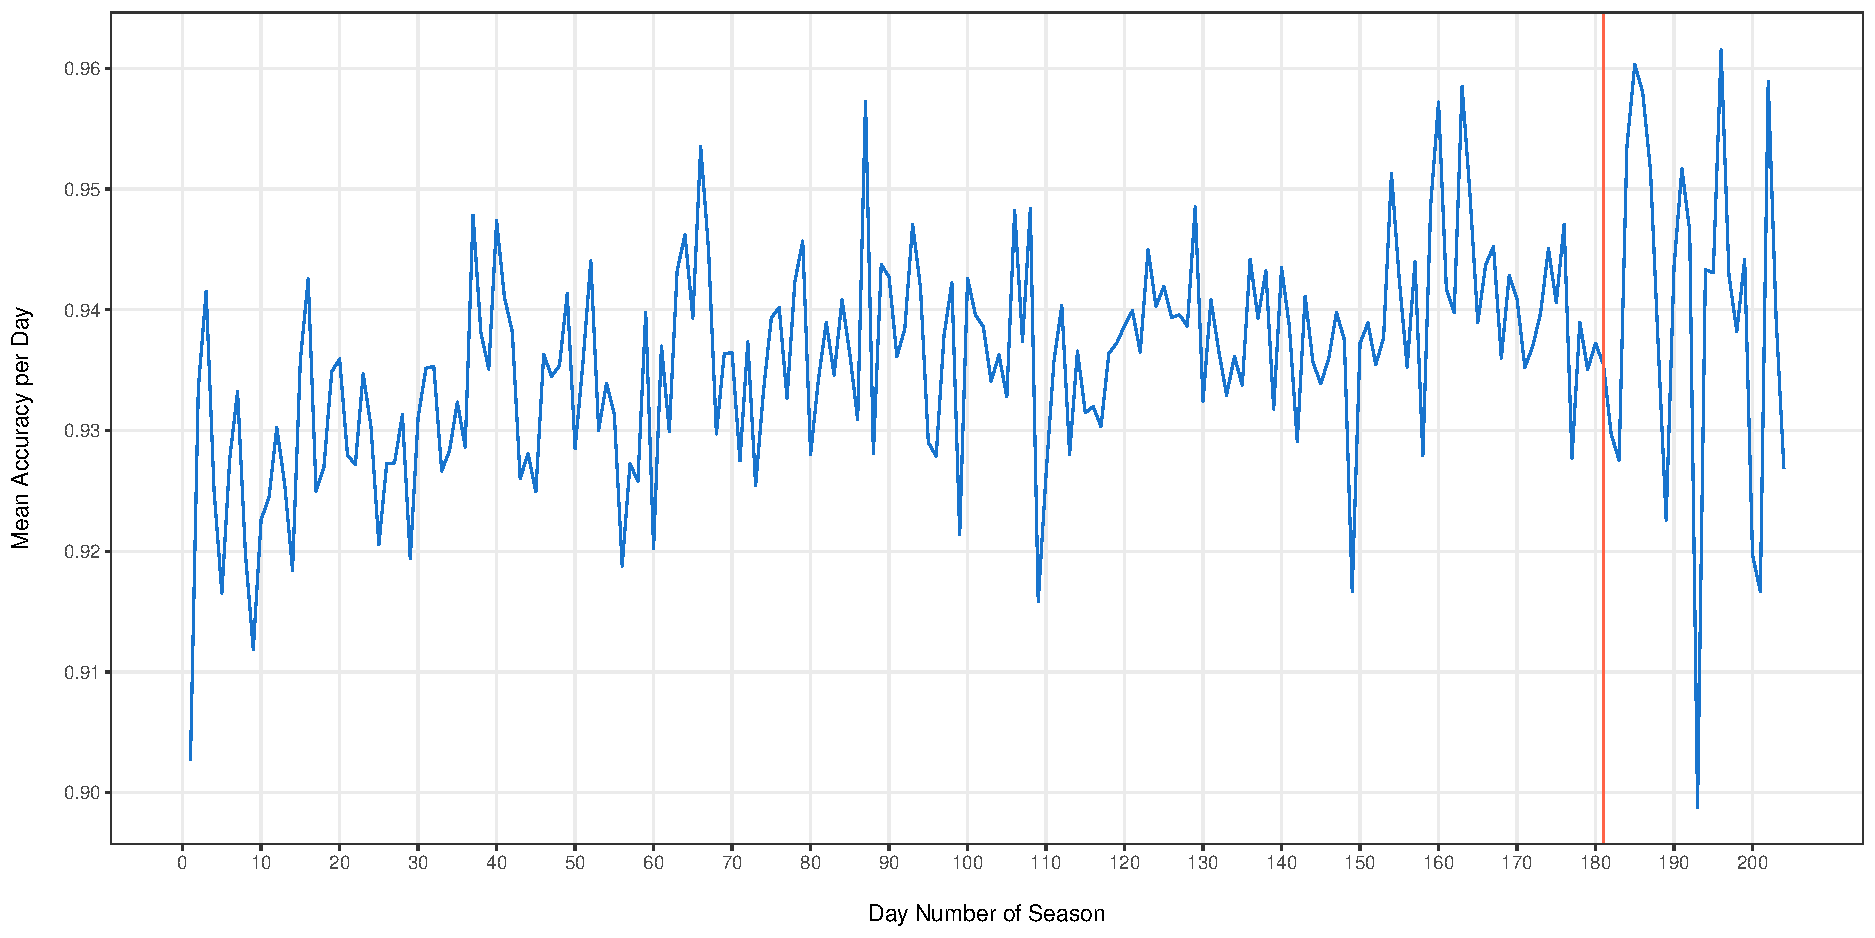
\includegraphics[width = 5in]{../figs/ump_acc_season.pdf}
\end{center}

\end{frame}

\section{Questions?}\label{questions}

\begin{frame}{Contact Details}

\begin{center}
{\Large{\bf{Aaron R. Baggett, Ph.D.}}}

{\small{Assistant Professor of Psychology\\
University of Mary Hardin-Baylor\\
{\large{\faEnvelope}} \url{abaggett@umhb.edu}\\
{\large{\faPhone}} (254) 295-4553\\
{\large{\faTwitter}} \href{http://twitter.com/aaron_baggett}{@aaron\_baggett}}}
\end{center}

\end{frame}

\end{document}
